% Created 2022-08-18 Thu 00:07
% Intended LaTeX compiler: pdflatex
\documentclass[11pt]{article}
\usepackage[utf8]{inputenc}
\usepackage[a4paper,margin=1.5in]{geometry}
\usepackage[T1]{fontenc}
\usepackage{graphicx}
\usepackage{grffile}
\usepackage{longtable}
\usepackage{wrapfig}
\usepackage{rotating}
\usepackage[normalem]{ulem}
\usepackage{amsmath}
\usepackage{textcomp}
\usepackage{amssymb}
\usepackage{capt-of}
\usepackage{hyperref}
\newcommand{\qed}{\mbox{}\hspace*{\fill}\nolinebreak\mbox{$\rule{0.6em}{0.6em}$}}
\date{}
\title{Floyd's cycle detection algorithm}
\hypersetup{
 pdfauthor={},
 pdftitle={Floyd's cycle detection algorithm},
 pdfkeywords={},
 pdfsubject={},
 pdfcreator={Emacs 27.1 (Org mode 9.3)}, 
 pdflang={English}}
\begin{document}

\maketitle
\section{Why the tortoise and rabbit meet?}
\begin{itemize}
    \item Imagine a loop (and nothing else) of \(n\) nodes so it's a polygon with n
vertices.
    \item Place the tortoise and the rabbit on any two nodes of your choice.
    \item The key is to not really number any of the nodes so they are
        indistinguishable.
    \item Now, let the distance between the rabbit and the tortoise be \(d\)
        hops.
    \item At each step, the tortoise moves to the adjacent node, while the
        rabbit hops two nodes. Now since the nodes are indistinguishable, we can
        place ourselves in the frame of reference of the tortoise.
    \item Then, from the perspective of the tortoise, after each step the
        tortoise remains where it was while the rabbit moves one hop closer to
        the tortoise.
    \item Thus the sequence of distances eventually approaches 0 (\(\{d, d-1,
        d-2,\dotsc,1,0\}\).
    \item So, whenever tortoise and rabbit enter the same loop, they'll
        definitely meet at some point.
    \item QED \qed
\end{itemize}
\section{Where do they meet?}
\begin{centering}
    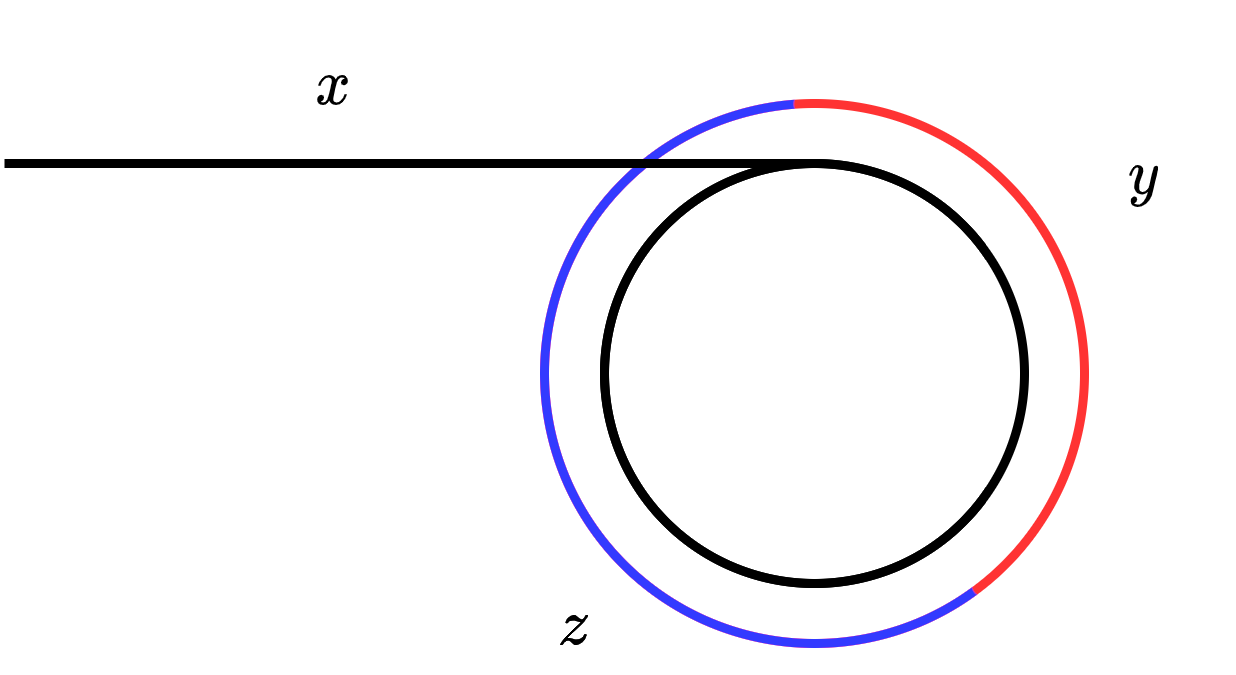
\includegraphics[width=0.9\textwidth]{/home/mridul/exdir/floyd_cycle/floyd.png}
\end{centering}
\begin{itemize}
    \item Begin by looking at the above diagram. \(x\) is the non cycle
        distance, \(y\) is where in the cycle rabbit and tortoise meet, \(z\) is
        the rest (distance left to start of the cycle).
    \item When the two meet, tortoise covers \(x+\lambda_1 n+y\) distance for
        some \(\lambda_1\) (where distance is number of nodes they hop on).
        \(\lambda_1\) represents the number of times the two go around the cycle
        from the start to meet at \(y\). \\ Note: \(\lambda_1\le 1\). Why?
    \item Also, rabbit covers \(x+\lambda_2 n+y\).
    \item Since rabbit moves at twice the speed of tortoise: 
        \begin{align*}
            &\quad\;\; 2(x+\lambda_1 n+y)\;=x+\lambda_2 n +y\\
            &\Rightarrow 2x+2\lambda_1 n+2y=x+\lambda_2 n+y\\
            &\Rightarrow x = \lambda n - y\text{, where
            }\lambda=\lambda_2-\lambda_1\text{ and since
            }\lambda_2\ge\lambda_1\text{, }\lambda\ge 0.\\
        \end{align*}
    \item Now, let \(x=\alpha n+\beta\), then:
        \begin{align*}
            &\quad\;\;x\operatorname{mod} n=-y\operatorname{mod} n=z\operatorname{mod} n\\
            &\Rightarrow\beta\operatorname{mod} n = \;\;z\operatorname{mod} n\\
            &\quad\;\;\text{and since both }\beta<n\text{ and }z<n\text{ the equality
            holds without ``mod''}\\
            &\Rightarrow\beta = z
        \end{align*}
    \item What this means is we can move one of the pointers to the head of the
        LL while leave the other at the meeting point (and we no longer
        distinguish between tortoise or rabbit, they are both tortoise now.)
        Then we can start both of these moving one hop at a time. The one at the
        head will move \(\alpha n\) times \(\beta=z\) will be left in the non
        cycle segment, while the one inside the cycle will move in cycles
        \(alpha\) times and stay at the location \(y\) in the loop with \(z\)
        left. After next \(\beta=z\) moves, the two will meet again at the
        beginning of the loop.\qed
\end{itemize}
\end{document}
